

\documentclass[12pt, a4paper]{article}


\usepackage{fancyhdr, enumerate}
\usepackage{amssymb}
\usepackage{geometry, amsmath, amsfonts, float, graphicx}
\usepackage{gensymb}
\usepackage{hyperref, listings}
\usepackage{matlab-prettifier}
\usepackage{caption}
\geometry{
	top=0.9in,           
	inner=0.6in,
	outer=0.6in,
	bottom=2in,
	tmargin= 10ex,       
	headsep=0.6cm,          
}
\pagestyle{fancy}

\fancyhead{}
\fancyfoot{}

\fancyhead[L]{Bioen 316 AC \\Homework 5\\ May 17, 2019}
\fancyhead[R]{Skyler Hallinan\\ hallisky@uw.edu \\ 1732227}

\lstMakeShortInline[style=Matlab-editor]"
\begin{document}
\vspace*{-3mm}
\section*{Problem 1} 
Use the convolution integral to find the convolution result $y(t) = u(t) * e^{-t} u(t)$ where $x * h$ represents the convolution of $x$ and $h$, and $u(t)$ is the piecewise unit step function, defined as   \begin{align*}
    u(t) &= \begin{cases}
      1, & t > 0 \\
      0, & t < 0
    \end{cases}
  \end{align*}\\
\textbf{Answer: } \\
We rewrite our convolution $y(t) = u(t) * e^{-t} u(t)$ as follows:
\begin{align*}
y(t) = \int_{-\infty}^{\infty} u(t- \tau) u(\tau) e^{-\tau} d\tau
\end{align*}
The unit step function $u(\tau)$ is 0 for all $\tau <0$, so we can set our lower bound to 0. In addition, our unit step function $u(t-\tau)$ is 0 for all $\tau > t$, so we can set our upper bound to $t$. After changing these bounds, we can replace these unit step functions with the value 1. Then we have:
\begin{align*}
y(t) &= \int_{0}^{t} u(t- \tau) u(\tau) e^{-\tau} d\tau \\
&= \int_{0}^{t} e^{-\tau} d\tau \\
&= \left [- e^{-\tau} |_{0}^{t} \right ] \\
y(t) &= 1- e^{-t}
\end{align*}
We see the result of the integral is $y(t) = 1- e^{-t}$. However, we must multiply by the unit step function $u(t)$, because we created a limit on $t$ when we used $t$ to to set a limit on $\tau$. Then, we finally have:
\begin{align*}
y(t) &= u(t)(1- e^{-t}) \\
    y(t) &= \begin{cases}
      1-e^{-t}, & t > 0 \\
      0, & t < 0
    \end{cases}
\end{align*}
\section*{Problem 2: Derivative \& high pass filter circuits}
The circuit shown here acts as a first-order high pass filter. Note that the capacitor is in series with R1, in the input path. In contrast, if this were a low-pass filter, the capacitor would be in parallel with Rf. You may ignore the resistor at the non-inverting input. It does have a practical purpose in a real circuit, but it does not appear in our calculations.
\begin{figure}[H]
\centering
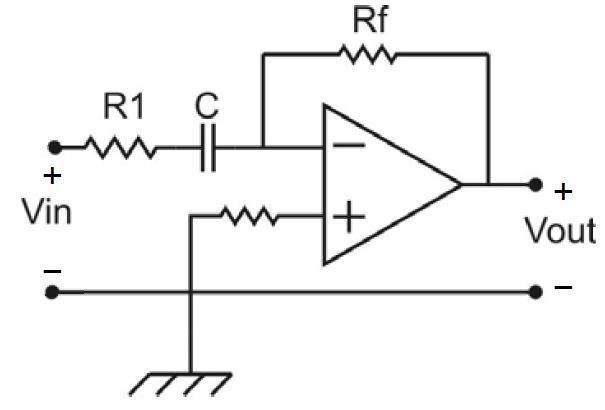
\includegraphics[width=0.5\textwidth]{circ1}
\caption{Image of the circuit}
\end{figure}
\begin{enumerate}[(a)]
\item Use impedance methods and your knowledge of inverting op-amp circuits to derive this circuit’s complex gain function, $G(\omega) = \frac{V_{out}(\omega)}{V_{in}(\omega)}$ \\ \\
\textbf{Answer: } \\
In an inverting op-amp circuit, we have the following relationships:
\begin{align*}
G(\omega) = \frac{V_{out}(\omega)}{V_{in}(\omega)} = -\frac{R_f}{R_1 +C} &= -\frac{R_f}{R_1 + \frac{1}{j\omega C}} =  -\frac{R_f j \omega C}{R_1 j \omega C + 1} \\
|G (\omega) | &= \sqrt{\frac{(R_f\omega C)^2}{(R_1\omega C)^2 + 1}}
\end{align*}
\item Determine the cutoff frequency and pass-band gain, and sketch a Bode magnitude plot. \\ \\
\textbf{Answer: } \\
The cutoff frequency for this active filter is achieved when the magnitude of our complex gain, $|G(\omega)|$ is equal to $\frac{1}{\sqrt{2}}$. Since we also have an amplification element in our gain function with a constant ratio of $\frac{R_f}{R_1}$, along with the attenuation at specific frequencies (since this is a high pass filter), we multiply this by our normal cutoff gain ratio, $\frac{1}{\sqrt{2}}$, and solve for when our $\omega$ meets this:
\begin{align*}
|G (\omega_{cutoff}) | &= \sqrt{\frac{(R_f\omega_{cutoff} C)^2}{(R_1\omega_{cutoff} C)^2 + 1}} = \frac{1}{\sqrt{2}} \cdot \frac{R_f}{R_1}\\
\frac{(R_f\omega_{cutoff} C)^2}{(R_1\omega_{cutoff} C)^2 + 1} &= \frac{R_f^2}{2R_1^2} \\
2R_1^2(R_f\omega_{cutoff} C)^2 &= R_f^2\left [(R_1\omega_{cutoff} C)^2 + 1 \right ] \\
2R_1^2 \omega_{cutoff}^2C^2  &=R_1^2\omega_{cutoff}^2 C^2 + 1 \\
R_1^2 C^2 \omega_{cutoff}^2 &= 1 \\
\omega_{cutoff} &= \frac{1}{R_1 C_1}
\end{align*}
The passband gain is the difference between the highest and lowest gain achievable. We see:
\begin{align*}
\lim_{\omega \to \infty} |G(\omega)| = \frac{R_f}{R_1}, \quad \lim_{\omega \to 0} |G(\omega)| = 0
\end{align*}
Therefore our pass band gain is $\frac{R_f}{R_1} - 0 = \frac{R_f}{R_1}$. The bode plot of this circuit is attached to a separate sheet.
\item Remove resistor $R_1$ and show, using time-domain math, that the resulting circuit
produces some constant times the derivative $\frac{dV_{in}}{dt}$, so it is an inverting differentiator \\ \\
\textbf{Answer: } \\
\begin{align*}
I_{in} = I_{f}, &\quad I_f = -\frac{V_{out}}{R_f} &\text{Ohm's Law, Circuit Fact} \\
Q = C V_{in} \quad &\Rightarrow \quad \frac{dQ}{dt} = C \frac{d V_{in}}{dt} \quad \Rightarrow \quad I_{in} = C \frac{dV_{in}}{dt} \\
-\frac{V_{out}}{R_f} = C \frac{dV_{in}}{dt} \quad &\Rightarrow \quad V_{out} = -R_f C \frac{dV_{in}}{dt}
\end{align*}
\end{enumerate}
\section*{Problem 3: Inductor-based Integrator}
Start with the inverting differentiator that has one capacitor and one resistor, then replace
the capacitor with an inductor L, named for Heinrich (Henry) Lenz.
\begin{enumerate}[(a)]
\item Derive the time-domain input/output function to show that the output voltage is an
integral of the input voltage. \\ \\
\textbf{Answer: } \\
We use similar substitutions to get the following:
\begin{align*}
I_{in} = I_{f}, &\quad  I_f = -\frac{V_{out}}{R_f} &\text{Ohm's Law} \\
V_{in} = L \frac{dI_{in}}{dt} \quad &\Rightarrow \quad I_{in} = \int \frac{V_{in}}{L} dt \\
-\frac{V_{out}}{R_f} &= \int \frac{V_{in}}{L} dt \\
V_{out} &= -\frac{R_f}{L} \int V_{in} dt
\end{align*}
\item Assuming an ideal inductor, what is the impulse response of this circuit?\\ \\
\textbf{Answer:} \\
Our input voltage is now the impulse response, and our output voltage is directly related to the integral of this input. We note that the integral of a single unit impulse is the unit step function $u(t)$. Then we see:
\begin{align*}
V_{out} &= -\frac{R_f}{L} \int \delta(t) dt \\
&= -\frac{R_f}{L} u(t) \\
   V_{out} &= \begin{cases}
      -\frac{R_f}{L}, & t > 0 \\
      0, & t < 0
    \end{cases}
\end{align*}
\item One drawback of using an inductor in place of a capacitor is that inductors are larger,
but that is not the only drawback. Assuming an ideal inductor, about how much more
power does an inductor-based integrator consume (convert to heat) than a capacitor-based
integrator in response to a unit impulse input? You may write value this in terms
of R, L, and C, assuming the same R in both circuits. \\ \\
\textbf{Answer: } \\
First, we define the unit impulse function:
\begin{align*}
    \delta(t) &= \begin{cases}
    	\infty, & t = 0 \\
      0, & t \neq 0
    \end{cases}
\end{align*}
We first calculate the power dissipated in our integrator circuit. We note that since we have an ideal inductor, there will be no power dissipated (converted to heat) by the inductor, as there is no resistance in an ideal capacitor, and $P(t) = \frac{\Delta v(t)^2}{R}$. However, there will be power dissipated by the resistor in our circuit. \\ \\
We see that the current in our inductor can be given by $i_L = \int \frac{V_{in}}{L} dt$ which is the same current as through the resistor. In addition, our $V_{in} = \delta(t)$. We also see from above that with this unit impulse, the $V_{out}$ is $\frac{R_f}{L}u(t)$. Finally, we see that the formula for power dissipated through our resistor is $P(t) = \Delta v(t) i(t)$:
\begin{align*}
V_{in} = \delta(t), \quad V_{out} = \frac{R_f}{L}u(t), &\quad P(t) = \Delta v(t) i(t), \quad i_L = \int \frac{V_{in}}{L} dt \\
i_L = \int \frac{V_{in}}{L} dt =\int \frac{\delta(t)}{L} dt \quad &\Rightarrow \quad i_L = \frac{1}{L} u(t)  \\
 P(t) = \Delta v(t) i(t) = \frac{R_f}{L}u(t) \cdot \frac{1}{L} u(t) \quad &\Rightarrow \quad P(t) = \frac{Rf}{L^2} u(t)^2 \\
    P(t) &= \begin{cases}
      \frac{R_f}{L^2}, & t > 0 \\
      0, & t < 0
    \end{cases}
\end{align*}
Then we calculate the power in our capacitor circuit (once again, our input voltage is $\delta(t)$, the unit impulse):
\begin{align*}
V_{out} = -R_f C \frac{d \delta(t)}{dt}, \quad V_{in} &= \delta(t), \quad I_f = \frac{V_{out}}{R_f} \\
V_{out} &= -R_f C \frac{d \delta(t)}{dt} \\
&=  -R_f C \delta(t) \\
P(t) = \Delta v(t) i(t) &= -R_f C \delta(t) \cdot \frac{ -R_f C \delta(t)}{R_f} = R_f C^2 \delta(t)^2 \\
    P(t) &= \begin{cases}
      R_f C^2, & t > 0 \\
      0, & t < 0
    \end{cases}
\end{align*}
Therefore our power dissipated in a capacitor circuit of this type (with $t>0$) is equal to $R_f C^2$, while in an inductor circuit of this type, it is equal to $\frac{R_f}{L^2}$. Therefore our dissipated power difference going from capacitor to inductor is $\Delta P = R_f C^2 - \frac{R_f}{L^2}$ for $t > 0$ (and 0 for $t \neq 0$).
\item Inductors are generally not ideal, having some finite resistance. How does the
existence of this parasitic resistance affect the behavior of our “integrator” circuit?
Support your answer with hand-drawn sketches of the new impulse response (i.e., the
output voltage, $v(t)_{out}$ when the input is a delta function) and the relationship of $V(j\omega)_{out}$ to $V(j\omega)_{in}$ in a rough Bode plot. \\ \\
\textbf{Answer: } \\
We see that with a parasitic resistance, we get the following complex gain:
\begin{align*}
G(j\omega) = \frac{R_f}{R_{parasitic} + L} &= \frac{R_f}{R_{parasitic} + j\omega L} = \frac{\frac{R_f}{j\omega}}{\frac{R_{parasitic}}{j\omega} + 1} \\ 
|G(j\omega)| &= \sqrt{\frac{\frac{R_f}{\omega}^2}{\frac{R_{parasitic}}{\omega}^2 + 1}} \\
\lim_{\omega \to 0} |G(j\omega)|  = \frac{R_f}{R_{parasitic}}, &\quad \lim_{\omega \to \infty} |G(j\omega)|  = 0
\end{align*}
Therefore we see that the gain as $\omega$ approaches 0 is no longer $\infty$; it is now equal to $\frac{R_f}{R_{parasitic}}$. We now effectively have a low pass filter. \\ \\
Then we look at how our $v_{out}$ changes. We solve the following ODE:
\begin{align*}
\frac{d v_{out}}{d t}+\frac{R_{p}}{L} v_{out} &=-\frac{R_{f}}{L} v_{i n} &\text{$v_{out}$ relation with parasitic resistance}\\
\mu(t) &= e^{\int{\frac{R_p}{L}} dt} = e^{\frac{R_p}{L}t} &\text{Let integration constant be 0}\\
\mu(t) \left [ \frac{d v_{out}}{d t}+\frac{R_{p}}{L} v_{out} \right ] &= -\mu(t) \frac{R_{f}}{L} v_{i n} &\text{Multiply by integrating factor} \\
 \frac{d}{dt}(e^{\frac{R_p}{L}t} v_{out}) &=  -e^{\frac{R_p}{L}t} \frac{R_{f}}{L} v_{i n} \\
v_{out} &= \frac{\int -e^{\frac{R_p}{L}t} \frac{R_{f}}{L} v_{i n} dt}{e^{\frac{R_p}{L}t} } \\
&= \frac{-\frac{R_f}{L}\frac{L}{R_p} v_{in} e^{\frac{R_p}{L}t} + C}{e^{\frac{R_p}{L}t}}\\
&= -\frac{R_f}{R_p}v_{in} + \frac{C}{e^{\frac{R_p}{L}t}}
\end{align*}
Then, we solve for $C$. We see that the impulse response of a system is its transient response. Therefore, we see that $v_{in} = 0$, and the initial condition $v_{out}(0) = \frac{-R_f}{L}$, the value of the output voltage produced by applying an impulse function $\delta(t)$ to the circuit:
\begin{align*}
v_{out} &= -\frac{R_f}{R_p}v_{in} + \frac{C}{e^{\frac{R_p}{L}t}} \\ 
v_{out}(0) = -\frac{R_f}{L} &= -\frac{R_f}{R_p}(0) + \frac{C}{e^{\frac{R_p}{L} (0)}} &\text{Initial condition: t=0} \\
-\frac{R_f}{L} = \frac{C}{1} \quad &\Rightarrow \quad C = -\frac{R_f}{L}
\end{align*}
Thus, we have our final solution of:
\begin{align*}
v_{out} &= -\frac{R_f}{R_p}v_{in} - \frac{R_f}{Le^{\frac{R_p}{L}t}}
\end{align*}
For plotting, see attached page.
\end{enumerate}
\section*{Problem 4: \textit{What is it?}}
Start with the standard inverting amplifier shown in figure 12.9 of the textbook. Replace $R_f$ with a diode that permits current to flow from the op-amp inverting input to the op-amp
output, but not from output to input. Recall that the voltage-current relationship for a
diode is $i = I_s e^{\lambda v}$, where $v= $ forward voltage and $\lambda = \frac{q}{kT}$, where $q$ is the charge of one electron, $k$ is Boltzmann's constant, $T$ is temperature, and $I_s$ is the ``reverse current'' which
is in the range of 10 - 100 nA, but you can leave it as $I_s$.
\begin{enumerate}[(a)]
\item Derive the mathematical function that relates $v_{out}$ to $v_{in}$ for this peculiar circuit. \\ \\
\textbf{Answer: } \\
See attached page for circuit diagram of 4. From the circuit diagram, we see that we can derive $v_{out}$ as follows:
\begin{align*}
V^{-} = V^{+} = 0 &\Rightarrow i^{-} = i^{+} = 0 \\
i_{in} &= - i_{out} &\text{Previous line knowledge, Kirchhoff's Rule}\\
\frac{V_{in}}{R_1} + I_s e^{\lambda v_{out}} = 0 \quad &\Rightarrow \quad -\frac{V_{in}}{R_1} = I_s e^{\lambda v_{out}}  &\text{General circuit voltages via Ohm's Law} \\
 \quad -\frac{V_{in}}{R_1 I_s} &= e^{\lambda v_{out}} \\
v_{out} &= \frac{\ln(-\frac{V_{in}}{R_1 I_s})}{\lambda} \\
&=  \frac{kT \ln(-\frac{V_{in}}{R_1 I_s})}{q}
\end{align*}
\item Draw a circuit that could be used to multiply two signals. My circuit involves four op-amps.
You do not need to derive the exact relationship between $v_{out}$ and $v_{in}$ for the
entire circuit, but do state the function of each op-amp sub-circuit. \\ \\
\textbf{Answer: } \\
See attached page.
\end{enumerate}
\end{document}